\part{Ecphoric Reconstruction}

\chapter{The Ecphoric Interaction Operator}\label{ch:ecphoric}

Recall is defined in this monograph as a conditional dynamical process and not as a ranking. Given a cue $c_t$, persistent memory $M_t$, a context $Z_t$, and the current field and phase state $\Psi_t$, the reconstruction is
\begin{equation}\label{eq:ecphoric}
r_t=\Eph(c_t,M_t,Z_t,\Psi_t),
\end{equation}
where $\Eph$ is realized as the terminal state of a reconstruction trajectory $r^{(0)},r^{(1)},\dots$ generated by an iteration $r^{(k+1)}=\mathcal T(r^{(k)},c_t,M_t,Z_t,\Theta^{(k)})$, with $\Eph$ the limit when it exists and the stopped iterate $r^{(K)}$ under a budget otherwise. The explicit trajectory, as opposed to a single ranking operation, has three uses. It makes the dependence on the dynamical state, the phases in particular, an object of analysis instead of a hidden implementation detail. It allows the intermediate states to be inspected, which is how false attractors and premature convergence are diagnosed. And it allows the cost of recollection to be accounted for as the number of steps and the work per step, which is the quantity that Chapter~\ref{ch:amortized} trades against accuracy.

The first question is under what conditions a partial cue initiates convergence toward the historically associated state. Let $x^\star$ denote the target, the organization that the trace was formed to preserve, and suppose that for a fixed cue the iteration is a self-map $F_c(\cdot)=\mathcal T(\cdot,c,M,Z,\Theta)$ of a complete metric space with Lipschitz constant $\lambda<1$ in its first argument. Then there is a unique fixed point $r^\star(c)$ and geometric convergence, and two statements bear on the target.

\begin{theorem}[Convergence to a cue-determined state and its distance from the target]\label{thm:converge}
Let $F_c$ be a $\lambda$-contraction on a complete metric space $(\mathcal R,d)$ with $\lambda<1$. Then (i) $F_c$ has a unique fixed point $r^\star(c)$ and $d(r^{(k)},r^\star)\le\frac{\lambda^k}{1-\lambda}d(r^{(1)},r^{(0)})$ for every initialization; (ii) for every $x\in\mathcal R$, $d(x,r^\star)\le d(x,F_c(x))/(1-\lambda)$, so the distance from the fixed point to the target is bounded by the residual $d(x^\star,F_c(x^\star))$ of the target under the cue-driven map; and (iii) if $c\mapsto F_c(r)$ is $L_c$-Lipschitz uniformly in $r$, then $d(r^\star(c),r^\star(c'))\le\frac{L_c}{1-\lambda}\,d(c,c')$.
\end{theorem}

\begin{proof}
Part (i) is the Banach fixed-point theorem with its standard a priori estimate. For (ii), $d(x,r^\star)\le d(x,F(x))+d(F(x),F(r^\star))\le d(x,F(x))+\lambda d(x,r^\star)$ and rearrangement gives the bound. For (iii), $d(r^\star(c),r^\star(c'))=d(F_c(r^\star(c)),F_{c'}(r^\star(c')))\le d(F_c(r^\star(c)),F_{c'}(r^\star(c)))+d(F_{c'}(r^\star(c)),F_{c'}(r^\star(c')))\le L_cd(c,c')+\lambda d(r^\star(c),r^\star(c'))$.
\end{proof}

Part (ii) is the precise sense in which a cue initiates convergence toward an historically associated state: the cue-driven map must have the target as an approximate fixed point, with residual small relative to $1-\lambda$. Contraction ensures convergence to a fixed point and says nothing by itself about whether that fixed point is the target; the answer is entirely in the residual. Part (iii) gives the stability of recollection under cue perturbation, so that small changes of the cue produce small changes of the reconstruction, with a constant that blows up as $\lambda\to1$. A cue that is too weak or too ambiguous makes the residual large, and then the unique fixed point may lie far from the target, which is the formal content of a spurious recollection.

\chapter{Associative Completion and Attractor Geometry}\label{ch:attractor}

Completion from incomplete observations is modeled by recurrent dynamics whose fixed points are intended to coincide with stored patterns. The continuous associative memory of Ramsauer and colleagues provides the cleanest instance for the purposes of analysis \cite{ramsauer2021}. For stored unit traces $m_1,\dots,m_P$ in the realified space and an inverse temperature $\beta>0$, the update map is
\begin{equation}\label{eq:modernhop}
F(r)=\sum_{i=1}^Pw_i(r)\,m_i,\qquad w_i(r)=\frac{e^{\beta\ip{m_i}{r}}}{\sum_je^{\beta\ip{m_j}{r}}},
\end{equation}
with $\ip{\cdot}{\cdot}$ the real inner product, and its stationary points are those of the energy $\mathcal E(r)=\frac12\norm r^2-\beta^{-1}\log\sum_je^{\beta\ip{m_j}{r}}$, since $\nabla\mathcal E(r)=r-F(r)$. The relation of this update to Bayesian reconstruction is stated in Proposition~\ref{prop:map}, where it appears as a monotone algorithm for a posterior mode. The geometry of the basins can be described directly. Fixed-point, limit-cycle, and metastable attractors need to be distinguished. A fixed point corresponds to a single stable reconstruction. A limit cycle, which cannot occur for the gradient dynamics above but can occur with the non-gradient terms of Chapter~\ref{ch:cgl}, corresponds to a recollection that is a cyclically evolving state, which may represent a temporally extended episode replayed in a loop. A metastable attractor is a state in which the dynamics lingers for a long time before leaving, and corresponds to an uncommitted or blended recollection.

\begin{proposition}[Basin condition and one-step cleanup]\label{prop:basin}
Let $\norm r\le1$ and suppose that for some index $1$ one has $\ip{m_1}{r}\ge\ip{m_i}{r}+\Delta$ for all $i\ne1$. Then the weight mass outside trace $1$ satisfies $\varepsilon:=\sum_{i\ne1}w_i(r)\le(P-1)e^{-\beta\Delta}$ and
\begin{equation}
\norm{F(r)-m_1}\le2\varepsilon\le2(P-1)e^{-\beta\Delta}.
\end{equation}
Moreover, with $\mu=\max_{i\ne j}\ip{m_i}{m_j}<1$, the gap at the new state satisfies $\ip{m_1}{F(r)}-\ip{m_i}{F(r)}\ge(1-\mu)-\varepsilon(3-\mu)$ for each $i\ne1$.
\end{proposition}

\begin{proof}
Each $w_i/w_1=e^{\beta(\ip{m_i}{r}-\ip{m_1}{r})}\le e^{-\beta\Delta}$ for $i\ne1$, so $\varepsilon=\sum_{i\ne1}w_i\le(1-\varepsilon)(P-1)e^{-\beta\Delta}\le(P-1)e^{-\beta\Delta}$. Then $F(r)-m_1=\sum_{i\ne1}w_i(m_i-m_1)$ and $\norm{m_i-m_1}\le2$. For the gap, $\ip{m_1-m_i}{F(r)}=\sum_jw_j\ip{m_1-m_i}{m_j}\ge w_1(1-\mu)-\sum_{j\ne1}w_j\cdot2\ge(1-\varepsilon)(1-\mu)-2\varepsilon$, using $\ip{m_1-m_i}{m_j}\ge-2$ for the remaining terms and $\ip{m_1-m_i}{m_1}=1-\ip{m_i}{m_1}\ge1-\mu$.
\end{proof}

The proposition says that if a state is separated from competitors by a margin $\Delta$ larger than $\beta^{-1}\log(P-1)$ by a sufficient amount, then one update step places the state within an exponentially small distance of the stored trace, and the margin at the new state is of the order of $1-\mu$, which exceeds the original margin requirement. The corresponding cue thresholds follow: the cue must supply enough correlation with the target trace, relative to its correlation with all other traces, to exceed $\beta^{-1}\log\bigl((P-1)/\varepsilon\bigr)$. False attractors arise in two ways. At low $\beta$ the weights are nearly uniform for a wide range of states, $F(r)$ approaches the mean of the traces, and the dynamics has a blend state near the centroid of the store; as $\beta$ increases this state loses stability through the criterion of Theorem~\ref{thm:contract} of Chapter~\ref{ch:stability} and is replaced by metastable states between clusters of similar traces and finally by single-trace attractors. At any $\beta$, spurious mixtures of traces with high mutual overlap are stable, because a state equidistant from two near-duplicates cannot be resolved by a margin. Spurious recollections in the sense of the previous chapter are the fixed points that are not near any stored trace, and their presence as a function of $\beta$, $P$, and the overlap structure is the object of the capacity analysis in Chapter~\ref{ch:capacity}.

Figure~\ref{fig:basin} plots the observed one-step error against the margin for cues of increasing corruption. Every observation lies below the bound, which is loose by a modest factor in the exponentially small regime, and the error stays near its maximum until the margin exceeds $\beta^{-1}\ln(P-1)$.

\begin{figure}[t]
\centering
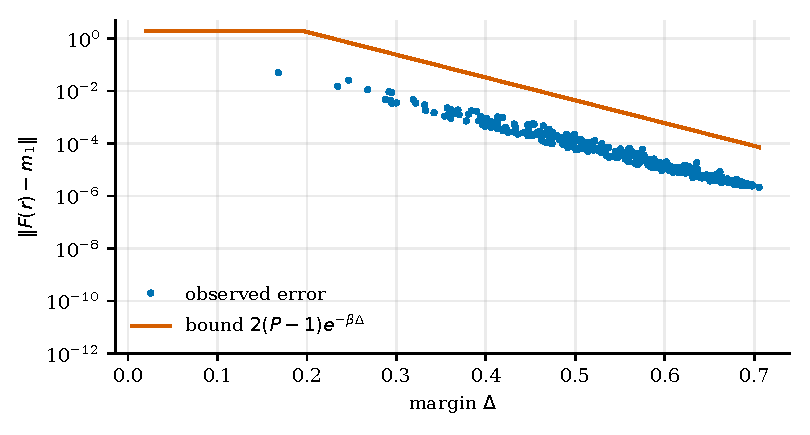
\includegraphics[width=0.85\textwidth]{figs/basin}
\caption{One-step cleanup error of the softmax update against the margin $\Delta$ for $P=50$ random unit traces in $\R^{64}$ and $\beta=20$, with the bound of Proposition~\ref{prop:basin}. Computed by the script \texttt{figs.py} with seed 8; an illustration of the stated analytic result and not an evaluation of the architecture.}\label{fig:basin}
\end{figure}

\chapter{Episodic Memory and Temporal Reinstatement}\label{ch:episodic}

Episodes are represented as trajectories and not as isolated vectors:
\begin{equation}\label{eq:episode}
e_i=\{x_i(\tau):\tau\in[t_i^-,t_i^+]\},
\end{equation}
where $x_i(\tau)$ is the organized state of the episode at internal time $\tau$. The difference between recovering what happened and recovering how it was organized in time is the difference between the content of an episode and its temporal organization. For a finite episode, content is the set or multiset of states visited, and temporal organization comprises the order in which they were visited, the intervals between them, the nesting of subepisodes, and the boundaries. Proposition~\ref{prop:nonimpl} showed that the two come apart in the encoding. They come apart in evaluation as well, which requires separate error measures. Let $x$ and $\hat x$ be a true and a reconstructed episode with item sequences $\sigma,\hat\sigma$ over a common item set. A content error is a distance between the multisets, for example the symmetric difference size. An order error is the normalized Kendall tau distance $\tau_K(\sigma,\hat\sigma)=\binom{n}{2}^{-1}\#\{\text{discordant pairs}\}$. An interval error is the root-mean-square difference of inter-item lags. A boundary error compares the sets of boundary times, for example by the F-score of boundaries matched within a tolerance. A reconstruction with zero content error and large order error is possible and is the expected failure of an encoding that stores a bag of items.

Event boundaries are defined here by a surprise criterion that follows the event-segmentation tradition in cognitive psychology \cite{zacks2007}: given a predictive model $p(x_{\tau+1}\mid x_{\le\tau})$, a boundary is placed at $\tau$ when $-\log p(x_{\tau+1}\mid x_{\le\tau})$ exceeds a threshold. Boundaries partition an episode into events and support two operations that matter for reconstruction: encoding at event level, in which each event is stored as a unit with within-event structure reconstructed from a generative model, and retrieval at event level, in which a cue first selects an event and then unfolds it. Temporal compression is the observation that recollection can proceed faster than the original episode. Let the replay map be $\tilde x(s)=x(\kappa s)$ with compression factor $\kappa>1$; for sampled trajectories this is subsampling or temporal pooling, and it reduces the cost of reconstruction by the factor $\kappa$ at the price of losing structure faster than the new sampling resolution, a loss that is bounded by the Nyquist condition on the retained structure.

Variable-resolution reconstruction is formalized by a nested family of subspaces $V_1\subseteq V_2\subseteq\cdots\subseteq V_L$ of the representation space and the corresponding orthogonal projections $\pi_\ell$. A reconstruction at level $\ell$ is $\pi_\ell\hat x$. Because the subspaces are nested, the squared error $\norm{x-\pi_\ell x}^2$ is nonincreasing in $\ell$, and the cost of reconstruction increases with $\ell$, so a coarse reconstruction at low cost can be refined as the task requires. The same family underlies the multiscale consolidation of Chapter~\ref{ch:consolidation}.

\chapter{Context-Sensitive Reconstruction}\label{ch:context}

Context is modeled as an operator acting on cues and candidate memories, so that the reconstruction under context $Z_t=z$ is
\begin{equation}\label{eq:context}
r_t=\Eph_{z}(c_t,M_t),
\end{equation}
where the operator $U_z$ acts on the cue before scoring and, in some formulations, on the stored traces as well. For a context group acting by unitary operators with $U_zU_{z'}=U_{z+z'}$, the effective score of a trace $m$ against a cue $c$ under context $z$ is $S(m,U_zc)$. This single construction accounts for four properties that are otherwise treated separately. Context-dependent accessibility arises because the score of a given trace against a given cue depends on $z$ through $U_z$. Cue ambiguity arises because the same $c$ under different contexts may match different traces. Competing interpretations arise because several $(m_i,z)$ pairs may give comparable scores. The effective retrieval landscape, the function $m\mapsto S(m,U_zc)$ over the store, changes with $z$ even though the store is unchanged.

Encoding specificity takes an exact form in the phase-context case. Let content be a unit vector $s$ and let the context be a global phase, $U_zs=e^{\iu z}s$.

\begin{proposition}[Encoding specificity as phase mismatch]\label{prop:encspec}
If a trace is stored as $m=U_{z_0}s$ and the cue is the same content presented under context $z$, $c=U_zs$, then $S(m,c)=\tfrac12\bigl(1+\cos(z-z_0)\bigr)$. The score equals one for matched context and zero for contexts differing by $\pi$, independent of the content.
\end{proposition}

\begin{proof}
Both vectors have unit norm, so by \eqref{eq:normalized} $S=\frac12(1+\Re\ip{e^{\iu z_0}s}{e^{\iu z}s})=\frac12(1+\Re e^{\iu(z-z_0)})$.
\end{proof}

The proposition formalizes the principle of Tulving and Thomson that the effectiveness of a retrieval cue depends on its overlap with the encoding context \cite{tulving1973}, with phase as the carrier of the context. Two corollaries follow from the structure of $U_z$. Because $U_z$ is invertible, the loss of accessibility caused by a context mismatch is not a loss of information: a system that can estimate the encoding context can undo the mismatch by applying $U_{z_0}U_z^{-1}$ to the cue, and the recovery of a trace by context reinstatement is exactly the application of this inverse. Second, when the context is not known, it can be marginalized or estimated: the posterior over context given the cue and the store is $p(z\mid c)\propto p(z)\sum_ie^{\beta S(m_i,U_zc)}$, and the system may either report the retrieval under the maximum a posteriori context or retain the mixture. The second option is the one required for a faithful treatment of ambiguity, since a hard assignment of context discards the information that the cue was compatible with several.

\chapter{Recollection, Familiarity, and Source Discrimination}\label{ch:source}

Recognition of familiar content and recovery of its historical context are different operations and must be distinguishable in a formal account. Let each trace carry a content part $\psi_i$ and a context-and-provenance part $\kappa_i$ (Chapter~\ref{ch:substrate}). Familiarity is a function of the content scores alone, for example $f(c)=\max_iS(\psi_i,c)$ or a smooth maximum $\beta^{-1}\log\sum_ie^{\beta S(\psi_i,c)}$. Recollection involves, in addition, the scores of the context parts, and the recollective output is not merely a number but a reconstruction with an attribution of source and context.

\begin{proposition}[Content-only familiarity cannot discriminate source]\label{prop:source}
Suppose two traces have identical content $\psi_A=\psi_B$ and different context-provenance parts $\kappa_A\ne\kappa_B$. Then any familiarity function that depends on the trace set only through the content scores takes equal values on the two traces, and no such function can assign different support to the hypotheses that the content was encountered in context $A$ or in context $B$.
\end{proposition}

\begin{proof}
A function of $\{S(\psi_i,c)\}_i$ treats traces $A$ and $B$ symmetrically because their content scores coincide for every cue $c$.
\end{proof}

Source attribution requires scoring the provenance parts, and the natural construction is a posterior over sources. With provenance labels $\nu_i$ and trace weights $w_i$ from the retrieval stage, define the attribution distribution $p(\nu\mid c)=\sum_i w_i\mathbb 1[\nu_i=\nu]$, and define source-attribution confidence as the probability mass on the most probable source, with a margin over the second. Two failure types can then be separated: content retrieval that is accurate with source misattribution, in which the content weights concentrate on traces whose content matches but whose provenance label differs from the true source because the encoding contexts were similar or because the cue carries stronger contextual overlap with the wrong source, and source attribution that is accurate for a content that is wrongly reconstructed. Provenance reconstruction, as distinct from provenance lookup, is the process of inferring the context of the original event from the stored context parts and the current state, and it is subject to all the interference effects of Chapter~\ref{ch:interference}. The consequence for architecture is that the provenance part of a trace must be a first-class component of the stored record, and that source discrimination is a test on which static content-addressable stores fail by construction, which makes it a meaningful discriminating experiment in Chapter~\ref{ch:source-exp}.

\chapter{Memory Interference and False Recollection}\label{ch:interference}

Interference is the degradation of recollection of one item by the presence of others. Four varieties are distinguished: proactive interference, in which earlier traces degrade the acquisition or retrieval of later ones; retroactive interference, in which later traces degrade earlier ones; trace competition, in which several traces compete for the same cue; and source confusion, in which the content is retrieved with the wrong attribution. In the softmax retrieval model, the effect of an additional trace on the weight of a target is exact.

\begin{proposition}[Dilution by an added trace]\label{prop:dilution}
Let a store give a target trace weight $w_t=e^{\beta s_t}/Z$ with $Z=\sum_je^{\beta s_j}$, and add a trace with score $s_n$ against the same cue. The new weight is $w_t'=w_t\,Z/(Z+e^{\beta s_n})$, and the fractional loss $1-w_t'/w_t=e^{\beta s_n}/(Z+e^{\beta s_n})$ equals the weight that the new trace itself receives.
\end{proposition}

\begin{proof}
The partition function becomes $Z'=Z+e^{\beta s_n}$ and the numerator is unchanged.
\end{proof}

The proposition shows that the interference caused by a trace is proportional to the probability mass it captures, which is largest when its score approaches or exceeds the target's, and negligible when $\beta(s_n-s_t)$ is very negative. In this model proactive and retroactive interference are arithmetically the same at retrieval: the order of storage does not enter. Distinguishing them requires an additional mechanism that depends on age or on write order, such as the amplitude decay discussed in Chapter~\ref{ch:forgetting} through the balance factor $\rho$, or a write rule that orthogonalizes a new trace against existing ones, so that the proactive and retroactive effects are caused by different parts of the architecture and are separately identifiable.

False recollection is a reconstruction that matches strongly but is historically wrong. A classical case is the production of a critical lure after studying a list of its associates \cite{roediger1995}, and a model of the effect follows from the geometry of the store.

\begin{proposition}[Centroid lure]\label{prop:lure}
Let $m_1,\dots,m_P$ be unit vectors with common pairwise real inner product $\mu\in[0,1)$, and let $g=\frac1P\sum_im_i$. Then $\norm g^2=(1+(P-1)\mu)/P$ and the normalized centroid $\hat g=g/\norm g$ satisfies $\ip{\hat g}{m_j}=\sqrt{(1+(P-1)\mu)/P}=:\kappa_P<1$ for every $j$. For a reconstruction $r=\hat g$, $S(r,\hat g)=1>S(r,m_j)=\tfrac12(1+\kappa_P)$, so the lure resonates more strongly than any presented item.
\end{proposition}

\begin{proof}
$\norm g^2=P^{-2}\bigl(P+P(P-1)\mu\bigr)$ and $\ip g{m_j}=P^{-1}(1+(P-1)\mu)$, so $\ip{\hat g}{m_j}=\ip g{m_j}/\norm g=\sqrt{(1+(P-1)\mu)/P}$, which is below one because $\mu<1$. The scores follow from \eqref{eq:normalized}.
\end{proof}

The proposition shows that a high resonance score cannot by itself certify historical support, since a composite assembled from many traces can be closer to a hypothetical item than to any actual one. The architecture therefore requires a quantity that is separate from resonance and that measures support by the ledger of Chapter~\ref{ch:provenance}.

\begin{definition}[Resonance and historical support]\label{def:support}
Let a reconstruction $r$ be given with resonance $\mathrm{res}(r)=\max_iS(m_i,r)$ against the store and let the ledger $H$ contain the inscription records. The reconstruction is $\delta$-supported if there is an inscription record $h\in H$ with $d(r,\mathrm{dec}(h))\le\delta$, where $\mathrm{dec}(h)$ is the content recorded at inscription, and is a constructed reconstruction otherwise. A recollection is reported as supported only if it is $\delta$-supported or if it is declared as a composite with the identified supporting records and their weights.
\end{definition}

With this separation the model can report a highly resonant but constructed reconstruction as such, and the evaluation in Chapter~\ref{ch:source-exp} measures the false-recollection rate as the fraction of reported-supported recollections that fail the ledger check against the ground truth of the experiment.
